\documentclass[../slides.tex]{subfiles}
\begin{document}

\begin{frame}{Quellen}
    \begin{table}[]
        \begin{tabular}{|l|l|p{8cm}|}
        \hline
        \textbf{Abbildungen}    & \textbf{Datum}  & \textbf{Link}\\ \hline
        Abbildung \ref{fig:globalRev}    & (07.03.2024)  & {https://additive.industrie.de/news/wohlers-report-2023-additive-fertigung-legt-um-183-zu/}\\ \hline
        Abbildung \ref{fig:slm}         & (07.03.2024) & {https://www.wdoose.de/en/additive-fertigung/slm-selective-laser-melting/}\\ \hline
        Abbildung \ref{fig:post_processing} & (07.03.2024)& {https://www.unionfab.com/blog/2023/08/post-processing-methods-metal-3d-printing}\\ \hline
        Abbildung \ref{fig:schraubstock}    & (07.03.2024)& {https://mav.industrie.de/werkzeuge/innovativer-schraubstock-vereinfacht-5-achs-bearbeitung/}\\ \hline
        \end{tabular}
        \end{table}
\end{frame}

\begin{frame}{Zeitplan}
    \begin{figure}[]
        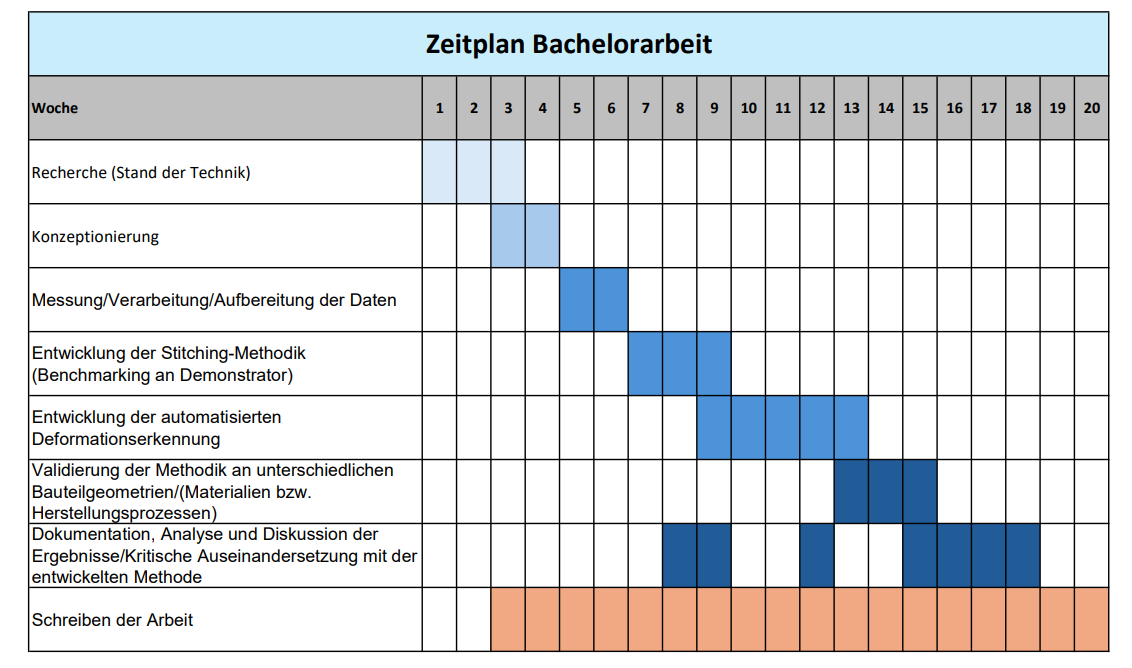
\includegraphics[height=185pt]{img_niklas/zeitplan.png}
        \caption[short]{Zeitplan}
        %
      \end{figure}
\end{frame}

\end{document}